\documentclass{elteikthesis}

\usepackage{tikz}
\usepackage{pgf-umlcd}
\usepackage{stuki}
\usepackage{ragged2e}
\usepackage{amssymb}
\usepackage{ucs}
\usepackage[utf8x]{inputenc}
\usepackage[english,hungarian]{babel}
\usepackage{graphicx}
\usepackage{pgfplots}

\renewcommand{\umlfillcolor}{white}
\renewcommand{\umldrawcolor}{black}
\renewcommand{\umltextcolor}{black}

\selectlanguage{hungarian}

\title{Függvény interpoláció megjelenítése}
\author{Szitár Gergő}
\supervisor{Dr. Krebsz Anna}
\supervisorstitle{egyetemi docens}
\period{Programtervező Informatikus BSc}
\thesisyear{2016}
\department{Numerikus Analízis tanszék}

\begin{document}

\frontmatter

	\maketitle
	\tableofcontents
	
\mainmatter

\chapter{Bevezetés}
\paragraph{}
A matematika segítségével változásokat, folyamatokat, tulajdonságokat megpróbál-juk függvények segítségével leírni, azonban a bonyolult függvények kiszámítása na-gyon költséges, polinom interpolációval egy közeli becslést tudunk kapni kisebb művelet-igénnyel. Ilyenkor megpróbál-unk közelíteni az eredeti függvényhez, ezt a módszert hívjuk interpolációnak.
\paragraph{}
A lényege, hogy mérések, mintavételezések segítségével bizonyos pontokban megha-tározzuk a függvény értékét, és ezen eredmények segítségével készítünk egy olyan függvényt, mely áthalad ezen pontokon. Vagyis egy olyan $I(x)$ függvény meghatározá-sa, melyre teljesül, hogy $I(x_i)=f(x_i)=y_i \; \forall i = 0\dots{n-1}$, ahol az $x_0, \dots, x_{n-1}$ pontok a mérések helyeit, továbbiakban alappontokat, és $y_0, \dots, y_{n-1}$ a mérések eredményét, vagyis az alappontokban az eredeti függvény által felvett értékeket jelölik.
\paragraph{}
Az előállított közelítési függvény típusa alapján három nagyobb csoportba sorolhat-juk a módszereket
\begin{itemize}
\item Polinomiálisak, ekkor az $n$ darab alappontra egy $n-1$-ed fokú polinomot illesztünk.
\item Trigonometrikusak, ekkor $sin$ és $cos$ függvények segítségével történik az interpol-áció. Periodicitásuk miatt hasznosak.
\item Racionális, ekkor két polinom hányadosaként adjuk meg a közelítése.
\end{itemize}
A továbbiakban csak a polinomiális módszerrel foglalkozunk tovább, hiszen ezen függvényeket adott pontban lineáris időben ki tudjuk értékelni.
\paragraph{}
A mai világban minden számítógépben megtalálható egy grafikus processzor, mely a képi megjelenítést teszi lehetővé. Ezt kihasználva, a szakdolgozat nem csak előállítja az a közelítést, hanem meg is jeleníti ezt. Egy dimenziós függvény esetében ez egy vonalat, két dimenziós esetén egy felszínt jelent.
\paragraph{}
Ehhez szükségünk van a létrejött függvényt számos sok pontban kiszámolnunk, a lineáris idejű kiértékelés biztosítja, hogy egy nem túl nagy fokszámú polinomot is viszonylag gyorsan meg tudjunk jeleníteni. Ezután a felhasználó már vizualizálva láthatja a függvény becslését, könnyebben fellelheti az érdekes, többi vizsgálatot megkövetelő részeket. Ilyenek lehetnek a szélső értékek, gyökök, más síkokkal vett metszéspontok.
\paragraph{}
Mindig is szerettem ötvözni más-más területen megszerzett tudásomat, így ebben a dolgozatban is ez a célom. A vizualizáció mindig is érdekelt, így a megjelenítés már adott volt. A matematikai háttér kisebb utána olvasás és kutatás után véglegesedett ki, hiszen az egyetem alatt csak egyváltozós függvények interpolációját tanultuk, de találtam módszereket az interpolációs polinom előállítására többváltozós függvények esetén. A matematikai függvényeket leíró formális nyelv átalakítása kiértékelhető formára hasonló elven működik, mint a fordítóprogramok működése. Így végül egy viszonylag komplex és sokrétegű programmal sikerült megoldani a kitűzött feladatot. További érdekes információkat a Tudományos háttér című fejezetben találhatnak, ahol részletes leírás található az egyes témakörökből.

\chapter{Tudományos háttér}
\section{Interpoláció}
\paragraph{}
A program polinom interpoláció felhasználásával készíti el a közelítést. Célja, hogy $n$ darab pontra egy $n-1$-ed fokú polinomot illesszen. Ezen függvények előnye, hogy kiszámításuk viszonylag olcsó, a Horner algoritmus felhasználásával lineáris időben ki lehet őket értékelni. Lentebb a két legnépszerűbb interpolációs polinom előállítását mutatom be. 
\subsection{Lagrange-interpoláció}
\paragraph{}
A módszer lényege, hogy $n$ darab különböző alappontból előállítunk egy polinom bázist, melyeket Lagrange alappolinomoknak nevezünk, és a lineáris kombinációjukkal előállítjuk a közelítő függvényt. Előnye a módszernek, hogy könnyen bővíthető több dimenzióra is, hátrá-nya a függvény kiértékelés magas költsége.
\paragraph{}
A bázis előállításához két követelményünk van:
\begin{itemize}
\item A $k$-adik bázis az $x_k$ alappontban 1 értéket vegyen fel.
\item A $k$-adik bázis az $x_i, i \neq k$ alappontokban pedig 0 értéket vegyen fel.
\end{itemize}
Formálisan felírva:
$$
	l_i(x_j) =
	\left\{
	  \begin{array}{lr}
	    0 & : i \neq j\\
	    1 & : i = j
	  \end{array}
	\right.
	\quad \forall i = 0\dots{n-1}
$$
Így egy olyan $n-1$ fokú polinomot kell előállítanunk, melynek ismerjük a gyökeit. Fel tudjuk írni a polinomot gyöktényezős alakban.
$$(x-x_0)\cdot(x-x_1)\cdots(x-x_{i-1})\cdot(x-x_{i+1})\cdots(x-x_{n-1})$$
Ezzel az első feltételt sikerült teljesíteni, ám az $x_i$ pontban felvett értéke még nem 1, ezért le kell osztanunk az ebben a pontban felvett értékkel.
$$(x_i-x_0)\cdot(x_i-x_1)\cdots(x_i-x_{i-1})\cdot(x_i-x_{i+1})\cdots(x_i-x_{n-1})$$
Sikerült is megkonstruálnunk azokat a bázis polinomokat, melyek megfelelnek a feltételeinknek. Kisebb átalakításokkal könnyen szorzat formára tudjuk hozni:
$$l_i(x) = \prod_{j = 0, j \neq i}^{n-1} \frac{x-x_j}{x_i-x_j}$$
\begin{center}
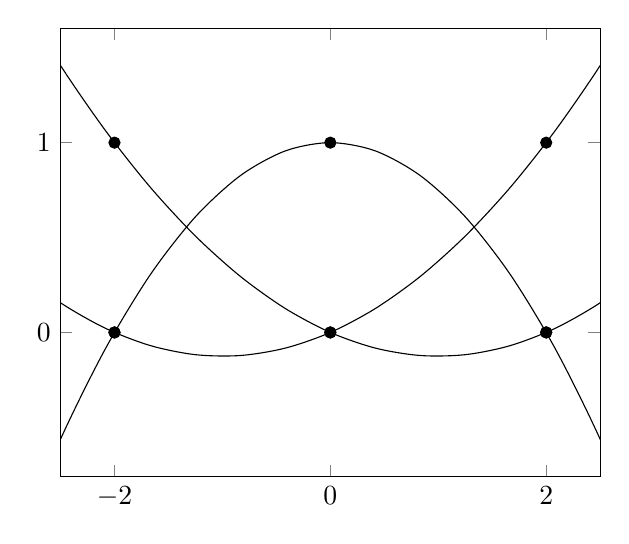
\begin{tikzpicture}
  \begin{axis}[
  	xmin=-2.5,
  	xmax=2.5,
  	xtick={-2,0,2},
  	ytick={0,1},
    xlabel={},
    ylabel={}
  ] 
    \addplot[only marks,black,samples at={-2,0,2}] {((x-0)*(x-2)/((-2-0)*(-2-2))};
    \addplot[smooth,mark=none,black] {((x-0)*(x-2)/((-2-0)*(-2-2))};
    
    \addplot[only marks,black,samples at={-2,0,2}] {((x+2)*(x-2)/((0+2)*(0-2))};
    \addplot[smooth,mark=none,black] {((x+2)*(x-2)/((0+2)*(0-2))};
    
    \addplot[only marks,black,samples at={-2,0,2}] {((x+2)*(x-0)/((2+2)*(2-0))};
    \addplot[smooth,mark=none,black] {((x+2)*(x-0)/((2+2)*(2-0))};
  \end{axis}
\end{tikzpicture} \\
{\footnotesize A bázispolinomok ábrázolva.}
\end{center}
\paragraph{}
Felhasználva az előbb készített bázist, és a függvény értékeket, az alábbi interpoláci-ós polinomot tudjuk előállítani:$$L(x) = \sum_{i=0}^{n-1} y_i \cdot l_i(x)$$
\begin{center}
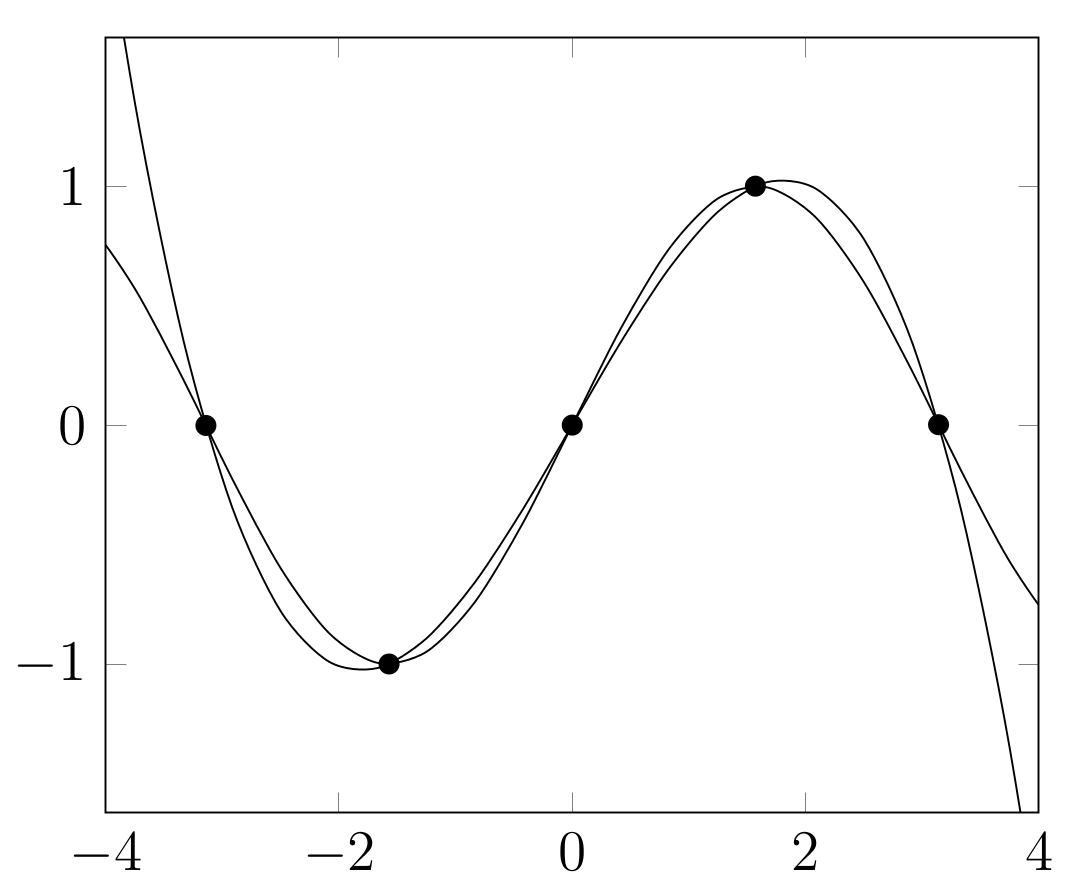
\includegraphics[width=10cm]{pics/polynomial_interpolation}\\
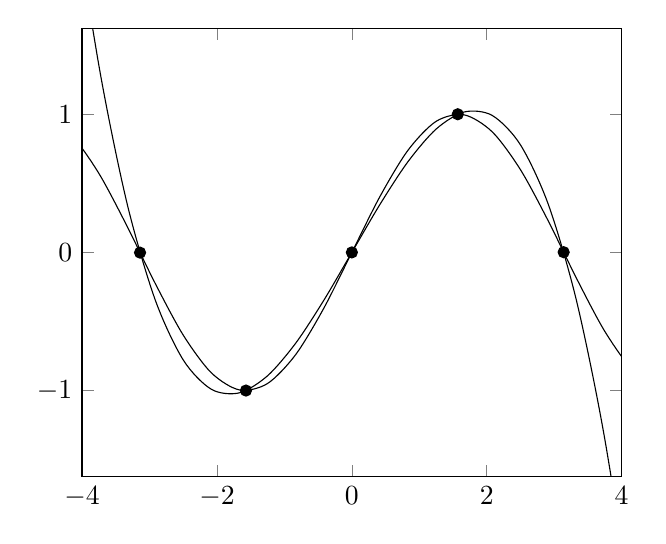
\begin{tikzpicture}
    \begin{axis}[xmin=-4,xmax=4, ]
        \addplot[only marks,black,samples at={-3.14,-1.57,0,1.57,3.14}] {sin(deg(x))};
        \addplot[smooth,mark=none,black] {sin(deg(x))};
        \addplot[smooth,mark=none,black] {(-2/pi)*(x+pi)+(4/(pi*pi))*(x+pi)*(x+pi/2)+(-8/(3*pi*pi*pi)*(x+pi)*(x+pi/2)*(x)};
    \end{axis}
\end{tikzpicture} \\
{\footnotesize Az interpolációs polinom és a függvény viszonya.}
\end{center}
\paragraph{}
Könnyen látható, hogy a fenti polinom teljesíti az interpolációs feltevést. $$L(x_i) = f(x_i) = y_i \quad \forall i = 0\dots{n-1}$$ Az interpolációs feltétel az $x_i$ pontban az, hogy $$P(x_i)=\sum_{j=0}^{n-1} y_j\cdot l_j(x_i) = y_i$$ Kiemelve a $j = i$ esetet a kapjuk, az alábbi alakot $$y_i \cdot l_i(x_i) + \sum_{j=0, i \neq j}^{n-1} y_j \cdot l_j(x_i)$$ Az $l_i(x)$ függvény készítésekor feltettük, hogy az $i$-edik alappontban az értéke legyen 1, minden más pontban 0. Ezt a behelyettesítést elvégezve, egy egyszerű formát kapunk. Innen triviálisan következik, hogy az interpolációs feltétel teljesül.
\paragraph{}
A fenti bázist fel tudjuk használni, hogy kiterjesszük az interpolációt kétváltozós függvényekre, egyetlen kikötés, hogy az alappontok egy rácsot alkossanak. Ez azt jelenti, hogy az x tengelyre levetítve kapjuk az $x_0, \dots, x_n$ felosztást, ugyanígy az $y$ tengelyre $y_0, \dots, y_m$. Ekkor feltétel, hogy $\forall (x_i, y_j) \; i = 0 \dots n, \; j = 0 \dots m$ pontban tudjuk a függvény értékét. Innen az egy változónál használt elvet követve, készítünk $(n+1) \cdot (m+1)$ darab bázist, melyek lineáris kombinációja fogja megadni az eredeti függvényt.
\begin{center}

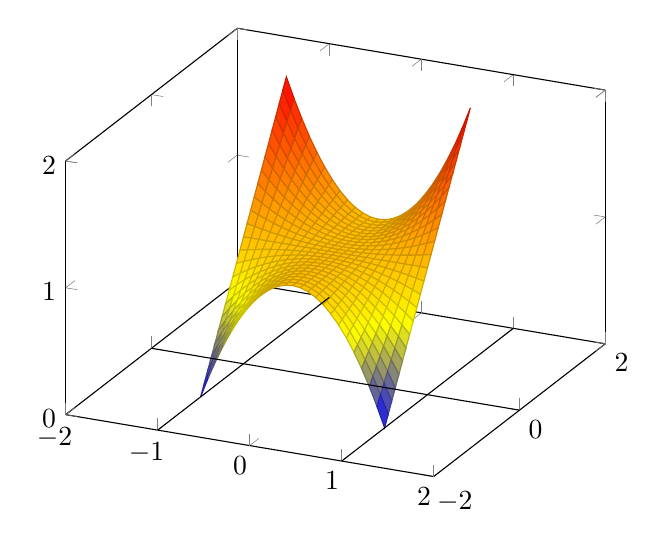
\begin{tikzpicture}
    \begin{axis}[xmin=-2,xmax=2,ymin=-2,ymax=2,zmin=0,zmax=2,smooth]
    	\addplot3[surf,domain=-1:1]{(x^2*y+1)};
        \addplot3[y domain=0:0,black,samples=10,domain=-2:2]({x},{0},{0});
    	\addplot3[y domain=0:0,black,samples=10,domain=-2:2]({1},{x},{0});
    	\addplot3[y domain=0:0,black,samples=10,domain=-2:2]({-1},{x},{0});
    \end{axis}
\end{tikzpicture} \\
{\footnotesize Mintavételezés rácspontokban.}

\end{center}
\paragraph{}
Olyan bázist keresünk, melyekkel fel tudjuk írni az interpolációs polinomot az alábbi formában.
$$L(x, y) = \sum_{i=0}^{n}\sum_{j=0}^{m}f(x_i, y_j) \cdot l_{i, j}(x, y)$$
Az $l_{i, j}(x,y)$ bázis elkészítéséhez fel tudjuk használni a már egy változónál elkészített bázis polinomokat. Legyen $$p_i(x) = \prod_{k = 0, k \neq i}^{n}\frac{x-x_k}{x_i-x_k},\; q_j(y) = \prod_{k = 0, k \neq j}^{n}\frac{y-y_k}{y_j-y_k}$$ A szorzatukból előáll a keresett bázis, hiszen az $l_{i, j}(x,y) = p_i(x)\cdot q_j(y)$ függvény az $(x_i, y_j)$ alappontban 1 értéket vesz fel, míg más alappontokban 0-át.
\subsection{Newton-féle interpolációs polinom}
\paragraph{}
Ez a módszer is egy polinom bázis lineáris kombinációjának segítségével alkotja meg a közelítést, viszont az együtthatók már nem a függvény értékek, hanem a belőlük előállított osztott differenciálok lesznek. Előnye a gyors számítás, az osztott differenciálok akár helyben is számolhatóak, új pont megadásakor nem kell teljesen újra számolni, elegendő csak az utolsó együtthatót kiszámolni. Hátránya, hogy nehe-zen terjeszthető ki több dimenzióra.
\paragraph{}
Először definiálnunk kell az osztott differenciált, $k$ darab pont osztott differenciál-jának a jelölése: $[y_0, \dots, y_{k-1}]$. Legyenek $x_0, \dots, x_n$ alappontok és $y_0, \dots, y_n$ értékek. Egy pontra az osztott differenciál értéke önmaga, vagyis $[y_k] := y_k$. Kettő vagy több pont esetén rekurzívan számoljuk ki.
$$[y_i, \dots, y_{i+j}] := \frac{[y_{i+1}, \dots, y_{i+j}] - [y_{i}, \dots, y_{i+j-1}]}{x_{j+i} - x_i}$$
A továbbiakban egy egyszerűbb jelölést vezetünk be abban az esetben, ha $y_i = f(x_i)$. Ekkor $[y_0, \dots, y_{k-1}]$ helyett $f[x_0, \dots, x_{k-1}]$ használható.
\begin{center}
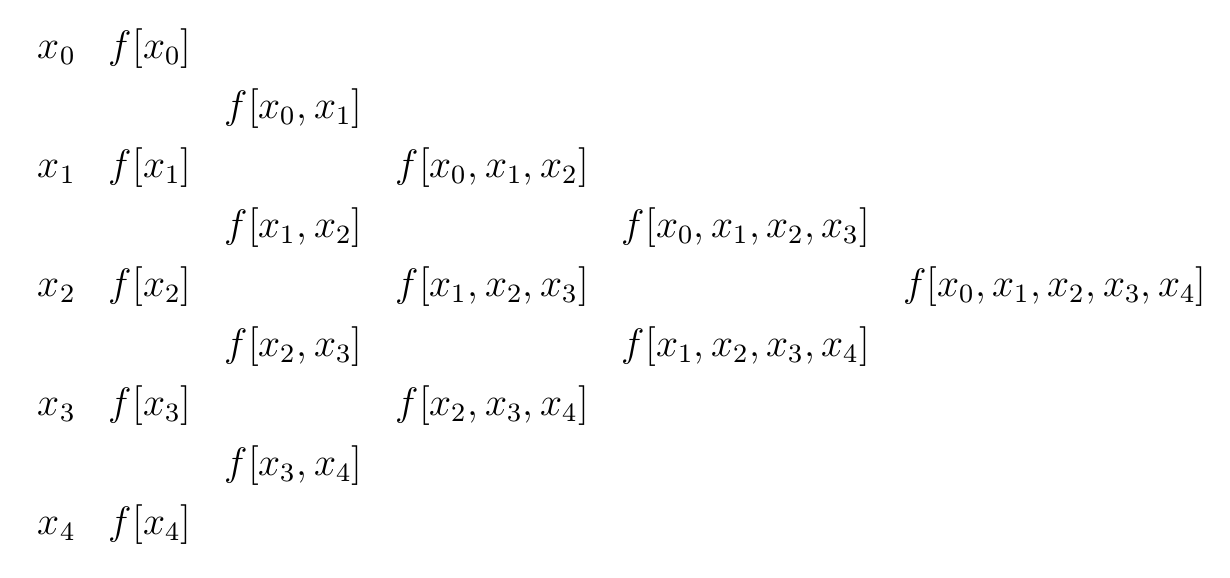
\includegraphics[width=15cm]{pics/divide_difference_table}\\
{\footnotesize Osztott differenciák táblázata.}
\end{center}
\paragraph{}
A bázis Lagrange módszerrel ellenkezően sokkal egyszerűbben felírható. Most a célunk egy könnyen bővíthető polinom bázis előállítása. Válasszuk az alábbi bázist. $$n_i = \prod_{j = 0}^{i}(x-x_j) \quad i \in [-1, n]$$
Ekkor felhasználva az osztott differenciált felírhatjuk az interpolációs polinomot egyszerű formában.
$$N(x) = \sum_{j=-1}^{n}a_j \cdot n_j(x), \quad \mbox{ahol} \; a_j = [y_0, \dots ,y_j]$$
\subsection{Alappontok}
\paragraph{}
Mivel adott $n$ darab pontra egyértelműen fel lehet írni egy $n-1$-ed fokú polinomot, ezért más technikához kell folyamodnunk, ha szeretnénk csökkentni a becslésünk hibáját. Egy bevált módszer, ha az alappontok megválasztásával próbáljuk csökkente-ni a hibát.
\paragraph{}
Vegyünk egy tetszőleges $f \in [a,b]^{n+1}$ függvényt, és közelítsük egy polinommal. Legyenek az alappontok $x_0, \dots, x_n$, ilyenkor egy tetszőleges belső pontban meg tudjuk becsülni a hibát. $$|f(x) - I_n(x)| \leq \frac{M_{n+1}}{(n+1)!} \cdot |\omega_n(x)|$$
$$M_{n+1} = \max |f^{n+1}(x)| \quad x \in [a,b]$$
$$\omega_n(x) = (x-x_0)\cdot(x-x_1)\cdots(x-x_n)$$
\paragraph{}
Azonban létezik megoldás ennek a hibának a lecsökkentésére, a Csebisev alappon-tok használatával. A Csebisev polinomok tulajdonsága, hogy minden gyöke a $[-1,1]$ intervallumon belül helyezkedik el és az $n$-edik polinomnak $n$ darab gyöke van.
\paragraph{}
Az $n$-edik előállítása megtörténhet rekurzióval , ekkor $T_0(x)=1$, $T_1(x) = x$ és $T_n(x) = 2x \cdot T_{n-1}(x)-T_{n-2}(x)$, vagy trigonometrikus függvények segítségével $T_n(x) = cos(n \cdot arccos(x))$.
\paragraph{}
Mivel a gyökök a $[-1, 1]$ intervallumon belül vannak, ezért lineáris transzformáció segítségével tudunk megfelelő alappontokat előállítani. Az $[a,b]$ intervallumra egy $f \in [-1,1] \rightarrow [a,b]$ függvény alkalmazásával tudjuk leképezni, mely $a$ és $b$ paraméter-ek segítségével az alábbi formában áll elő:
$$f(x) = \frac{a+b}{2}+\frac{b-a}{2} \cdot x$$
Elértük, hogy legyen $n$ darab alappontunk az $[a,b]$ intervallumon, melyekre el tudjuk így végezni az interpolációt. Ezekkel az alappontokkal készített polinom már sokkal jobb közelítést kapunk. $$|f(x)-I_n(x)| \leq \frac{M_{n+1}\cdot(b-a)^{n+1}}{(n+1)! \cdot 2^{2n+1}}$$
\paragraph{}
Ez annak a következménye, hogy $\omega_n(x)$ polinomnak a $0$-tól legkevésbé eltérő $1$ együtthatójú polinomot választjuk, mely a $T^*_n(x) = 2^{1-n} \cdot T_n(x)$. Ehhez a Csebisev polinom gyökei kell megválasztani alappontnak. Ezen polinomok tulajdonsága, hogy $\max |T^*_n(x)| = 2^{1-n} \quad x \in [-1,1]$. Le tudjuk vezetni, hiszen $T_n(x) = cos(n*arccos(x))$, így a szélső értéke $1$ lesz, $T^*_n(x)$ szélsőértéke pedig $2^{1-n}$.
Már csak a fenti $[-1,1] \rightarrow [a,b]$ transzformációt kell elvégeznünk, és az eredeti hibaképletben lévő $|\omega_n(x)|$ helyére behelyettesítve megkapjuk a fenti képletet.
\newpage
\section{3D grafika}
\subsection{Modellezés}
\subsection{Megjelenítés}
\newpage
\section{Formális nyelvek és fordító programok}
Matematika világában mindent megpróbálunk formálisan leírni, mert csak így tudjuk őket használni és bizonyítani. A nyelvekkel is ugyanígy járunk el, megpróbálunk szabályokat felírni, mely segítségével a nyelv levezethető. Ezzel el tudjuk dönteni, hogy egy adott szó, formális nyelvben vett szó, egy adott nyelvhez tartozik-e. Ez a folyamat történik akkor is, mikor a fordító program az általunk írt kódot elemzi és készíti el a futtatható állományt. Ekkor a programunk lesz a szó, és a fordítóprogram különböző elemzői döntik el, hogy valóban az adott programnyelvbe tartozik-e a kódunk.
\subsection{Nyelvek leírása formálisan}
\paragraph{}
A nyelvek alapjai a szimbólumok, a nem üres véges halmazuk pedig az ábécé. Egy $L$ ábécé feletti szavak halmazát $L^+$-al jelöljük, ha az üres szót is belevesszük, akkor $L^*$-al jelöljük.
\paragraph{}
Formális nyelveket le tudunk írni nyelvtanokkal, mely megadja a nyelv ábécéjét, terminális szimbólumok, és azokat a szabályokat, melyek segítségével az adott kezdő szimbólumból el tudunk jutni a nyelv által generált összes szóig. Továbbiakban $G$ nyelvtan egy olyan négyes $(N, T, P, S)$, ahol $T$ és $N$ a nemterminális és terminális szimbólumok ábécéi, feltétel, hogy diszjunktak. $P$ a szabályok halmaza, $(N \cup T)^+ \rightarrow (N \cup T)^*$ függvények, $S \in N$ pedig a kezdőszimbólum.
\paragraph{}
Az alábbi példán az egész számokon értelmezett összeadás és kivonás nyelvét mutatjuk be. Legyen $G=(N, T, P, S)$, ahol
$$
\begin{array}{rl}
T= & \{0, 1, 2, 3, 4, 5, 6, 7, 8, 9, +, -\} \\
N= & \{Start, Number, Digit, Operator\} \\
S= & Start \\
P= & \{Start \rightarrow Number | Number \; Operator \; Start, \\
&\; Number \rightarrow Digit | Digit \; Number, \\
&\; Digit \rightarrow 0 | 1 | 2 | 3 | 4 | 5 | 6 | 7 | 8 | 9, \\
&\; Operator \rightarrow + | -\}
\end{array}
$$
\paragraph{}
A szabályok alkalmazásával minden szóhoz elő tudunk állítani egy szintaxisfát, melynek a gyökerében a kezdőszimbólum, a leveleiben pedig nemterminális szimbólumok állnak. Ez a fa nem minden esetben egyértelmű, léteznek olyan szavak, melyekhez több fa is tartozik. Példákban a $1+2+3$ szóhoz két különböző fát tudunk előállítani, melyek később fontos szerepet töltenek be az elemzés során. Ilyenkor szükséges, hogy további elemzéshez a megfelelő fát küldjük tovább, a helyes eredmény érdekében.
\begin{center}
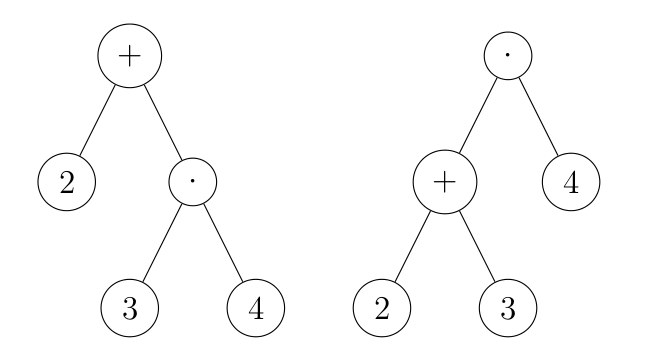
\includegraphics[width=5cm]{pics/syntax_tree}\\
{\footnotesize A $2+3+4$ kifejezés két szintaxisfája.}
\end{center}
\subsection{Fordítás menete}
\paragraph{}
A fordítás első lépése a lexikális elemzés, melynek feladata, hogy a bemenetről eldöntse, megfelel a nyelv ábécéjének, és szimbólumokra, úgynevezett tokenere bontsa azt. Ennek segítségére reguláris kifejezéseket használunk, melyekkel könnyen fel tudunk írni akár bonyolultabb szimbólumokat is.
\paragraph{}
Például a $(\backslash +|-)?[0-9]+(\backslash.[0-9]+)?$ kifejezés írja le a számokat. Három rész különböztethető meg, előjel, egészrész és törtrész. Az előjelet $(\backslash+|-)?$ írja le, ahol a $+$ és $-$ az előjeleknek felel meg, a $\backslash$ az úgynevezett escape karakter, a $+$ jelnek kitüntetett jelentése van. $|$ jelöli, hogy a kettő közül az egyik, ha többet írunk egymás utána, akkor a sok közül az egyiket jelenti. Sok elem esetén listát használhatunk, $[a-z]$, ez hasonló az előzőhöz, a sok elem közül az egyikre illeszkedik. A kifejezés végén álló $?$ az előtte álló részről megengedi, hogy nullaszor vagy egyszer szerepeljen. Hozzá hasonlóan a $+$ és $*$ jelek is a mennyiséget módosítják, míg a $+$ kifejezés egyszer vagy többször, addig a $*$ megengedi, hogy egyszer sem szerepeljen. A kifejezés $[0-9]+$ része a pozitív egész számokat írja le, az utolsó része pedig, hogy a pont után másik egész szám áll.
\paragraph{}
Miután a bemenetet tokenekre bontottuk, meg kell őket feleltetnünk a $P$ halmazban szereplő szabályoknak. Az $(X \rightarrow Y)$ szabály jelentése, hogy ha $X$-et le tudjuk vezetni, akkor $Y$-t is, ezt rekurzívan követve, ha egy szóról azt kapjuk, hogy $S$-ből levezethető, akkor a nyelv egyik szava. Könnyebb olvashatóság céljából, ha több olyan szabály létezik, mely bal oldala azonos, akkor őket össze tudjuk vonni, és a jobb oldalakat $|$-el elválasztva soroljuk fel.
\paragraph{}
Szemantikus elemzést azért végzünk, hogy az elkészített grammatika egyszerűbb legyen, és egyéb olyan feladatokat elvégezzünk, melyeket szükséges elvégezni, de a szintaktikus elemzéskor nem volt rá lehetőségünk. Kifejezések típusának helyességének ellenőrzése, újra deklarálás, vagy a nem deklarált változók tudjuk felismerése. Ezek egyszerű ellenőrzésének érdekében bevezetjük a szimbólumtáblát, mely feladata, hogy számon tartsa, mely függvények, változók vannak jelenleg definiálva, és mi az ő típusuk.
\paragraph{}
A lexikális, szintaktikus és szemantikus elemzés után már biztosítva van, hogy a fordítás lehetséges, ilyenkor az adott nyelvünket bizonyos szabályok alapján egy másik nyelvre tudjuk fordítani, mely lehet akár már futtatható kód, vagy még csak egy köztes nyelv, amiből egy másik fordítóprogram segítségével futtatható kódot kapunk.
\subsection{Matematikai függvények formális nyelve}
\paragraph{}
A függvények interpolációjához szükségünk van arra, hogy a programban a matematikai függvényeket feltudjuk ismerni, kitudjuk értékelni. Erre az előbb bemutatott formális nyelv modellt használjuk fel. Jelölje a $G=(N, T, P, S)$ a matematikai függvények nyelvét, már csak az egyes részeket kell definiálnunk.
\paragraph{}
Az ábécénk most tokenekből fog állni, melyekre illeszkedő reguláris kifejezéseket adunk meg.
$$T=\{var, num, open, close, add, min, mul, div, pow, abs, sin, cos, tg, ctg\}$$
Meg kell adnunk minden elemnek a reguláris kifejezését, azért, hogy a lexikális elemző fel tudja ismerni.
$$
\begin{array}{rlrl}
var & ::= x|y & num & ::= [0-9]+(\backslash.[0-9]+)? \\
open & ::= \backslash( & close & ::= \backslash)\\
add & ::= \backslash+ & min & ::= -\\
mul & ::= \backslash* & div & ::= \backslash\backslash\\
pow & ::= \wedge & abs & ::= abs\\
sin & ::= sin\ & cos & ::= cos\\
tg & ::= tg & ctg & ::= ctg
\end{array}
$$
Következő lépés, a szabályokban használt nemterminális szimbólumok megadása, ügyelve arra, hogy ezen halmaz metszete a terminális szimbólumok halmazával üres legyen.
$$N=\{Start, Binary, Unary, Expression\}$$
A nemterminális és terminális szimbólumok ismeretében meg tudjuk konstruálni a nyelv szabályait. Az $S=Start$ választásával, az alábbi formát ölti a nyelvtan:
$$
\begin{array}{rl}
P= & \{Start \rightarrow Expression, \\
&\; Expression \rightarrow open \; Expression \; close, \\
&\; Expression \rightarrow Binary \\
&\; Expression \rightarrow Unary \\
&\; Expression \rightarrow var \\
&\; Expression \rightarrow num \\
&\; Binary \rightarrow Expression \; add \; Expression \\
&\; Binary \rightarrow Expression \; min \; Expression \\
&\; Binary \rightarrow Expression \; mul \; Expression \\
&\; Binary \rightarrow Expression \; div \; Expression \\
&\; Binary \rightarrow Expression \; pow \; Expression \\
&\; Unary \rightarrow min \; Expression \\
&\; Unary \rightarrow abs \; Expression \\
&\; Unary \rightarrow sin \; Expression \\
&\; Unary \rightarrow cos \; Expression \\
&\; Unary \rightarrow tg \; Expression \\
&\; Unary \rightarrow ctg \; Expression\}
\end{array}
$$
A $var$ és $num$ tokeneket úgynevezett szemantikus értékkel is ellátjuk, itt tároljuk, hogy melyik változóról van szó, $x$ vagy $y$, illetve, hogy az adott számnak mi az értéke. A nyelvhez előre elkészített szimbólumtábla tartozik, melyben az egyes műveletek és függvények kiszámításának módja található. Megtalálható még benne az egyes bináris műveletek precedenciája, mely segít a helyes szintaxisfa előállításában.
\paragraph{}
Utolsó lépés az előállított fa segítségével kiértékelni a függvényt adott pontban. A mélységi bejárás algoritmusának postorder változatával könnyen el is tudjuk ezt végezni, hiszen szülő mindig egy részkifejezés főművelete, így azt az után kell elvégezni, hogy a gyerekeiben lévő műveletet elvégeztük. Egészen addig kell rekurzívan lefelé mennünk, amíg el nem érünk egy levélhez, ahol két lehetőség van. Az első, hogy a levélben egy változó van, ekkor a szemantikus érték alapján kiválasztjuk, hogy melyik változó értékét kell behelyettesíteni, a másik lehetőség, hogy egy szám áll ott, ilyenkor csak a szemantikus értékkel számolunk tovább.
\chapter{Felhasználói dokumentáció}
\section{Telepítés}
\section{Használat}
\section{Gyakran ismételt kérdések}

\chapter{Fejlesztői dokumentáció}
\section{Tervezés}
\subsection{Feladat specifikálása}
\subsection{Felhasználói esetek}
\subsection{Grafikus felület}
\section{Program felépítése}
\section{Osztályok leírása}
\subsection{Controller osztály}
\subsection{MainView osztály}
\subsection{OpenGLView osztály}
\subsection{Model osztály}
\section{Tesztelés}

\end{document}
